% Harmonic series convergence visualization
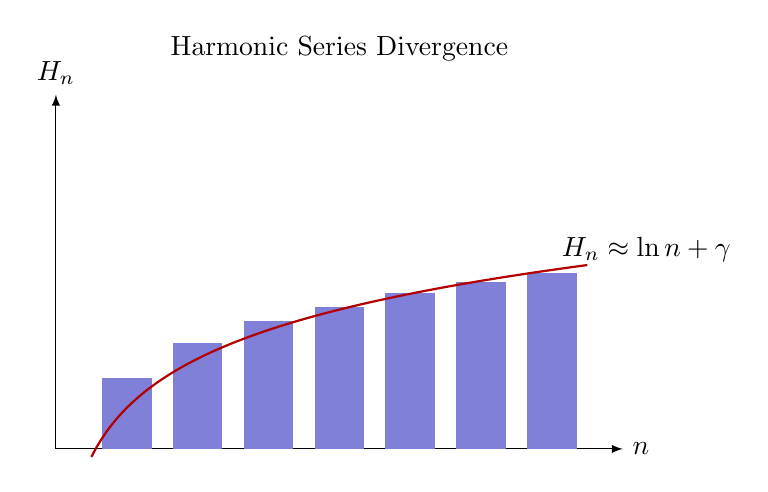
\begin{tikzpicture}[scale=0.9]
  % Axes
  \draw[->, >=latex] (0,0) -- (8,0) node[right] {$n$};
  \draw[->, >=latex] (0,0) -- (0,5) node[above] {$H_n$};
  
  % H_n bars (approximate)
  \foreach \n/\h in {1/1, 2/1.5, 3/1.8, 4/2, 5/2.2, 6/2.35, 7/2.48} {
    \fill[blue!70!black!50] (\n-0.35,0) rectangle (\n+0.35,\h);
  }
  
  % ln(n) curve
  \draw[red!70!black, thick, domain=0.5:7.5, samples=100] 
    plot (\x, {ln(\x) + 0.58});
  
  % Annotation
  \node[above right] at (7,2.5) {$H_n \approx \ln n + \gamma$};
  
  % Title
  \node[above=0.3cm] at (4,5) {Harmonic Series Divergence};
\end{tikzpicture}
